\documentclass[11pt,a4paper]{article}
\usepackage[utf8]{inputenc}
\usepackage[T1]{fontenc}
\usepackage{amsmath, amssymb, amsthm, bm}
\usepackage{geometry}
\usepackage{xcolor}
\usepackage{tcolorbox}
\usepackage{fancyhdr}
\usepackage{tikz}

\definecolor{myblue}{RGB}{0, 80, 150}
\definecolor{mygreen}{RGB}{34, 139, 34}

\newtcolorbox{terimbox}[1]{colback=blue!5!white,colframe=myblue,title=#1}
\newtcolorbox{theoriebox}[1]{colback=green!5!white,colframe=mygreen,title=\textbf{Özet ve Püf Noktalar: #1}}
\newtcolorbox{sonucbox}{colback=white,colframe=gray!50}

% NOTE: babel is intentionally NOT loaded (Turkish babel makes '=' active and breaks TikZ)

\geometry{margin=2.5cm}

\pagestyle{fancy}
\fancyhf{}
\fancyhead[L]{\textbf{Fizik 1 - Devoirs Maison}}
\fancyhead[R]{\textbf{DM1 \& DM2 Çözümleri}}
\fancyfoot[C]{\thepage}

\title{\textcolor{myblue}{\Huge\textbf{Fizik 1 - DM1 \& DM2}}\\[0.3cm]
\Large\textbf{Konu Anlatımlı ve Ayrıntılı Ödev Çözümleri}}
\author{}
\date{Ekim 2026}

\begin{document}

\maketitle
\tableofcontents
\newpage

%%%%%%%%%%%%%%%%%%%%%%%%%%%%%%%%%%%%%%%%%%%%%%%%%%%%%%%%%%%%%%%%%%%%%%%%%%%%%%%
% PARTIE 1 : DM1
%%%%%%%%%%%%%%%%%%%%%%%%%%%%%%%%%%%%%%%%%%%%%%%%%%%%%%%%%%%%%%%%%%%%%%%%%%%%%%%
\part*{DM 1 : Calcul Vectoriel et Systèmes de Coordonnées}
\addcontentsline{toc}{part}{DM 1 : Calcul Vectoriel et Systèmes de Coordonnées}

\begin{terimbox}{\textbf{Önemli Fransızca Fizik Terimleri (Terminologie Française - DM1)}}
\begin{itemize}
    \item \textbf{Vecteur unitaire:} Birim vektör (uzunluğu 1 olan vektör).
    \item \textbf{Produit scalaire / vectoriel / mixte:} Skaler / Vektörel / Karma çarpım.
    \item \textbf{Repère cartésien / cylindrique:} Kartezyen / Silindirik referans sistemi.
    \item \textbf{Dérivation des vecteurs:} Vektörlerin türevi (zincir kuralına dikkat).
    \item \textbf{Vecteur vitesse:} Hız vektörü (konumun türevi).
    \item \textbf{En déduire:} (Önceki bulgulardan) Yola çıkarak türetmek, çıkarmak.
    \item \textbf{Vérifier:} Doğrulamak, sağlama yapmak.
\end{itemize}
\end{terimbox}

\vspace{0.5cm}

\section*{Exercice 1 : Produits de vecteurs}

\begin{theoriebox}{Vektör Çarpımları ve Bazlar}
\begin{itemize}
    \item \textbf{Norm (Büyüklük):} Bir $\vec{v}$ vektörünün normu $||\vec{v}|| = \sqrt{v_x^2 + v_y^2 + v_z^2}$ formülü ile hesaplanır. Birim vektör ise $\vec{e_v} = \frac{\vec{v}}{||\vec{v}||}$ şeklinde bulunur.
    \item \textbf{Açılar:} İki birim vektörün \textit{skaler çarpımı} aradaki açının kosinüsünü verir ($\vec{e_1} \cdot \vec{e_2} = \cos\theta$). \textit{Vektörel çarpımının} normu ise sinüsünü verir ($||\vec{e_1} \times \vec{e_2}|| = \sin\theta$).
    \item \textbf{Baz Testi:} Üç vektörün bir baz oluşturması için lineer bağımsız olmaları gerekir. Bunun en kolay yolu \textit{determinantın} (karma çarpımın) $0$'dan farklı olduğunu göstermektir.
\end{itemize}
\end{theoriebox}

\subsection*{a) Calcul des normes et des vecteurs unitaires}
Soit les vecteurs $\vec{a}(1,2,2)$, $\vec{b}(2, 2\sqrt{2}, 2)$ et $\vec{c}(0, \sqrt{2}, \sqrt{2})$.
Leurs normes sont :
\begin{align*}
||\vec{a}|| &= \sqrt{1^2 + 2^2 + 2^2} = \sqrt{9} = 3 \\
||\vec{b}|| &= \sqrt{2^2 + (2\sqrt{2})^2 + 2^2} = \sqrt{4 + 8 + 4} = 4 \\
||\vec{c}|| &= \sqrt{0^2 + (\sqrt{2})^2 + (\sqrt{2})^2} = \sqrt{4} = 2
\end{align*}
Les vecteurs unitaires $\vec{e_v} = \frac{\vec{v}}{||\vec{v}||}$ correspondants sont :
\begin{sonucbox}
$\vec{e_a} = \left(\frac{1}{3}, \frac{2}{3}, \frac{2}{3}\right), \quad 
\vec{e_b} = \left(\frac{1}{2}, \frac{\sqrt{2}}{2}, \frac{1}{2}\right), \quad 
\vec{e_c} = \left(0, \frac{\sqrt{2}}{2}, \frac{\sqrt{2}}{2}\right)$
\end{sonucbox}

\subsection*{b) Calcul des cosinus des angles}
Le produit scalaire de deux vecteurs unitaires donne le cosinus de l'angle entre eux :
\begin{align*}
\cos\theta_a &= \vec{e_b} \cdot \vec{e_c} = \left(\frac{1}{2}\right)(0) + \left(\frac{\sqrt{2}}{2}\right)\left(\frac{\sqrt{2}}{2}\right) + \left(\frac{1}{2}\right)\left(\frac{\sqrt{2}}{2}\right) = \frac{2+\sqrt{2}}{4} \\
\cos\theta_b &= \vec{e_a} \cdot \vec{e_c} = \left(\frac{1}{3}\right)(0) + \left(\frac{2}{3}\right)\left(\frac{\sqrt{2}}{2}\right) + \left(\frac{2}{3}\right)\left(\frac{\sqrt{2}}{2}\right) = \frac{4\sqrt{2}}{6} = \frac{2\sqrt{2}}{3} \\
\cos\theta_c &= \vec{e_b} \cdot \vec{e_a} = \left(\frac{1}{2}\right)\left(\frac{1}{3}\right) + \left(\frac{\sqrt{2}}{2}\right)\left(\frac{2}{3}\right) + \left(\frac{1}{2}\right)\left(\frac{2}{3}\right) = \frac{1 + 2\sqrt{2} + 2}{6} = \frac{3+2\sqrt{2}}{6}
\end{align*}

\subsection*{c) Calcul des composantes des vecteurs (produits vectoriels)}
\begin{align*}
\vec{u_a} &= \vec{e_b} \times \vec{e_c} = 
\begin{vmatrix} 
\vec{i} & \vec{j} & \vec{k} \\ 
1/2 & \sqrt{2}/2 & 1/2 \\ 
0 & \sqrt{2}/2 & \sqrt{2}/2 
\end{vmatrix} 
= \vec{i}\left(\frac{2}{4} - \frac{\sqrt{2}}{4}\right) - \vec{j}\left(\frac{\sqrt{2}}{4} - 0\right) + \vec{k}\left(\frac{\sqrt{2}}{4} - 0\right) = \left( \frac{2-\sqrt{2}}{4}, -\frac{\sqrt{2}}{4}, \frac{\sqrt{2}}{4} \right) \\
\vec{u_b} &= \vec{e_c} \times \vec{e_a} = 
\begin{vmatrix} 
\vec{i} & \vec{j} & \vec{k} \\ 
0 & \sqrt{2}/2 & \sqrt{2}/2 \\ 
1/3 & 2/3 & 2/3 
\end{vmatrix} 
= \vec{i}\left(\frac{2\sqrt{2}}{6} - \frac{2\sqrt{2}}{6}\right) - \vec{j}\left(0 - \frac{\sqrt{2}}{6}\right) + \vec{k}\left(0 - \frac{\sqrt{2}}{6}\right) = \left( 0, \frac{\sqrt{2}}{6}, -\frac{\sqrt{2}}{6} \right) \\
\vec{u_c} &= \vec{e_a} \times \vec{e_b} = 
\begin{vmatrix} 
\vec{i} & \vec{j} & \vec{k} \\ 
1/3 & 2/3 & 2/3 \\ 
1/2 & \sqrt{2}/2 & 1/2 
\end{vmatrix} 
= \vec{i}\left(\frac{2}{6} - \frac{2\sqrt{2}}{6}\right) - \vec{j}\left(\frac{1}{6} - \frac{2}{6}\right) + \vec{k}\left(\frac{\sqrt{2}}{6} - \frac{2}{6}\right) = \left( \frac{2-2\sqrt{2}}{6}, \frac{1}{6}, \frac{\sqrt{2}-2}{6} \right)
\end{align*}

\subsection*{d) Déduction des sinus et vérification}
Puisque $||\vec{u}|| = ||\vec{e_1} \times \vec{e_2}|| = ||\vec{e_1}|| \cdot ||\vec{e_2}|| \cdot \sin\theta = \sin\theta$ :
\begin{align*}
\sin\theta_a &= ||\vec{u_a}|| = \sqrt{\left(\frac{2-\sqrt{2}}{4}\right)^2 + \left(-\frac{\sqrt{2}}{4}\right)^2 + \left(\frac{\sqrt{2}}{4}\right)^2} = \sqrt{\frac{10-4\sqrt{2}}{16}} = \frac{\sqrt{10-4\sqrt{2}}}{4} \\
\sin\theta_b &= ||\vec{u_b}|| = \sqrt{0 + \left(\frac{\sqrt{2}}{6}\right)^2 + \left(-\frac{\sqrt{2}}{6}\right)^2} = \sqrt{\frac{4}{36}} = \frac{1}{3} \\
\sin\theta_c &= ||\vec{u_c}|| = \sqrt{\left(\frac{2-2\sqrt{2}}{6}\right)^2 + \left(\frac{1}{6}\right)^2 + \left(\frac{\sqrt{2}-2}{6}\right)^2} = \frac{\sqrt{19-12\sqrt{2}}}{6}
\end{align*}

\textbf{Vérification à l'aide de la question b) :}
On utilise la relation trigonométrique $\sin\theta = \sqrt{1 - \cos^2\theta}$ :
\begin{itemize}
    \item Pour $\theta_a$ : $\cos\theta_a = \frac{2+\sqrt{2}}{4} \implies \cos^2\theta_a = \frac{6+4\sqrt{2}}{16}$. Donc $\sin\theta_a = \sqrt{1 - \frac{6+4\sqrt{2}}{16}} = \frac{\sqrt{10-4\sqrt{2}}}{4}$. (Vérifié)
    \item Pour $\theta_b$ : $\cos\theta_b = \frac{2\sqrt{2}}{3} \implies \cos^2\theta_b = \frac{8}{9}$. Donc $\sin\theta_b = \sqrt{1 - \frac{8}{9}} = \frac{1}{3}$. (Vérifié)
    \item Pour $\theta_c$ : $\cos\theta_c = \frac{3+2\sqrt{2}}{6} \implies \cos^2\theta_c = \frac{17+12\sqrt{2}}{36}$. Donc $\sin\theta_c = \sqrt{1 - \frac{17+12\sqrt{2}}{36}} = \frac{\sqrt{19-12\sqrt{2}}}{6}$. (Vérifié)
\end{itemize}

\subsection*{e) Base et base normée ?}
Pour que les trois vecteurs constituent une base de l'espace, ils doivent être non coplanaires. On vérifie cela en calculant leur produit mixte (le déterminant) :
$$ \det(\vec{u_a}, \vec{u_b}, \vec{u_c}) = 
\begin{vmatrix} 
\frac{2-\sqrt{2}}{4} & -\frac{\sqrt{2}}{4} & \frac{\sqrt{2}}{4} \\[2mm]
0 & \frac{\sqrt{2}}{6} & -\frac{\sqrt{2}}{6} \\[2mm]
\frac{2-2\sqrt{2}}{6} & \frac{1}{6} & \frac{\sqrt{2}-2}{6}
\end{vmatrix} 
$$
En développant par rapport à la première colonne (le terme central est nul car $a_{21}=0$) :
$$ \det = \frac{2-\sqrt{2}}{4}\, M_{11} + \frac{2-2\sqrt{2}}{6}\, M_{31} $$
avec les mineurs :
\begin{align*}
M_{11} &= \left(\frac{\sqrt{2}}{6}\right)\left(\frac{\sqrt{2}-2}{6}\right) - \left(-\frac{\sqrt{2}}{6}\right)\left(\frac{1}{6}\right) = \frac{2-2\sqrt{2}}{36} + \frac{\sqrt{2}}{36} = \frac{2-\sqrt{2}}{36} \\
M_{31} &= \left(-\frac{\sqrt{2}}{4}\right)\left(-\frac{\sqrt{2}}{6}\right) - \left(\frac{\sqrt{2}}{4}\right)\left(\frac{\sqrt{2}}{6}\right) = \frac{2}{24} - \frac{2}{24} = 0
\end{align*}
Donc :
$$ \det = \frac{2-\sqrt{2}}{4} \cdot \frac{2-\sqrt{2}}{36} = \frac{(2-\sqrt{2})^2}{144} = \frac{6-4\sqrt{2}}{144} \neq 0 $$
Puisque le déterminant est non nul, les vecteurs $\vec{u_a}, \vec{u_b}, \vec{u_c}$ \textbf{constituent bien une base}. 
Cependant, pour qu'une base soit normée, il faut que la norme de chaque vecteur soit égale à $1$. Or, d'après la question précédente, $||\vec{u_b}|| = \frac{1}{3} \neq 1$. Cette base \textbf{n'est donc pas normée}.

\newpage

\section*{Exercice 2 : Dérivation des vecteurs unitaires}

\begin{theoriebox}{Vektörlerin Türevi ve Dönen Referans Sistemleri}
\begin{itemize}
    \item \textbf{Zincir Kuralı:} Zamana ($t$) göre türev alırken, açının ($\varphi$) da zamanla değiştiğini hesaba katmalıyız: $\frac{d}{dt} = \frac{d\varphi}{dt} \frac{d}{d\varphi} = \dot{\varphi} \frac{d}{d\varphi}$
    \item \textbf{Kendine Diklik:} Her birim vektörün uzunluğu sabit ($1$) olduğundan, kendi türevi daima kendisine \textit{diktir}. 
    \item \textbf{Bağıl Türev:} Dönen silindirik sistemdeki ($R_{cyl}$) bir gözlemci, kendi eksenlerini ($\vec{e_\rho}, \vec{e_\varphi}$) dönmüyor olarak görür. Bu yüzden o referansta bu vektörlerin türevi $0$'dır.
\end{itemize}
\end{theoriebox}

\subsection*{a) Calcul des dérivées en projection dans la base cartésienne $B$}
Les vecteurs unitaires polaires s'écrivent dans la base cartésienne fixe $B (\vec{e_x}, \vec{e_y}, \vec{e_z})$ :
\begin{align*}
\vec{e_\rho} &= \cos\varphi \vec{e_x} + \sin\varphi \vec{e_y} \\
\vec{e_\varphi} &= -\sin\varphi \vec{e_x} + \cos\varphi \vec{e_y}
\end{align*}
Puisque les vecteurs $\vec{e_x}$ et $\vec{e_y}$ sont fixes dans le repère $R$, on dérive uniquement les coefficients par rapport à $\varphi$ :
\begin{sonucbox}
$$ \left[\frac{d\vec{e_\rho}}{d\varphi}\right]_R = \frac{d(\cos\varphi)}{d\varphi} \vec{e_x} + \frac{d(\sin\varphi)}{d\varphi} \vec{e_y} = -\sin\varphi \vec{e_x} + \cos\varphi \vec{e_y} $$
$$ \left[\frac{d\vec{e_\varphi}}{d\varphi}\right]_R = \frac{d(-\sin\varphi)}{d\varphi} \vec{e_x} + \frac{d(\cos\varphi)}{d\varphi} \vec{e_y} = -\cos\varphi \vec{e_x} - \sin\varphi \vec{e_y} $$
\end{sonucbox}

\subsection*{b) Expressions de ces dérivées dans la base cylindrique $B_{cyl}$}
Pour déduire les expressions dans la base cylindrique, on compare les résultats de la question (a) avec les définitions de $\vec{e_\rho}$ et $\vec{e_\varphi}$.
Pour la première dérivée, on reconnaît exactement l'expression de $\vec{e_\varphi}$ :
$$ -\sin\varphi \vec{e_x} + \cos\varphi \vec{e_y} = \vec{e_\varphi} $$
Pour la deuxième dérivée, en factorisant par le signe moins, on obtient :
$$ -\cos\varphi \vec{e_x} - \sin\varphi \vec{e_y} = -(\cos\varphi \vec{e_x} + \sin\varphi \vec{e_y}) = -\vec{e_\rho} $$
Ainsi, en projection dans la base $B_{cyl}$, on obtient :
\begin{sonucbox}
$$ \left[\frac{d\vec{e_\rho}}{d\varphi}\right]_R = \vec{e_\varphi} $$
$$ \left[\frac{d\vec{e_\varphi}}{d\varphi}\right]_R = -\vec{e_\rho} $$
\end{sonucbox}

\subsection*{c) Expressions par rapport au temps $t$}
Si $\varphi$ est fonction du temps, on applique la règle de la chaîne à l'aide des résultats de la question précédente :
\begin{sonucbox}
$$ \left[\frac{d\vec{e_\rho}}{dt}\right]_R = \left[\frac{d\vec{e_\rho}}{d\varphi}\right]_R \frac{d\varphi}{dt} = \frac{d\varphi}{dt} \vec{e_\varphi} $$
$$ \left[\frac{d\vec{e_\varphi}}{dt}\right]_R = \left[\frac{d\vec{e_\varphi}}{d\varphi}\right]_R \frac{d\varphi}{dt} = -\frac{d\varphi}{dt} \vec{e_\rho} $$
\end{sonucbox}

\subsection*{d) Propriété générale de la dérivée d'un vecteur unitaire}
\textbf{Démonstration :} Soit $\vec{u}$ un vecteur unitaire, donc son produit scalaire par lui-même est constant : $\vec{u} \cdot \vec{u} = 1$.
En dérivant cette relation par rapport au temps :
$$ \frac{d}{dt} (\vec{u} \cdot \vec{u}) = \frac{d\vec{u}}{dt} \cdot \vec{u} + \vec{u} \cdot \frac{d\vec{u}}{dt} = 2 \left( \vec{u} \cdot \frac{d\vec{u}}{dt} \right) = 0 $$
Le produit scalaire étant nul, la dérivée $\frac{d\vec{u}}{dt}$ est orthogonale à $\vec{u}$. Par conséquent, la dérivée de tout vecteur unitaire n'a aucune composante sur lui-même.

\subsection*{e) Le vecteur rotation $\vec{\Omega}$}
On cherche un vecteur $\vec{\Omega} = \Omega_\rho \vec{e_\rho} + \Omega_\varphi \vec{e_\varphi} + \Omega_z \vec{e_z}$ tel que :
$\left[\frac{d\vec{e_\rho}}{dt}\right]_R = \vec{\Omega} \times \vec{e_\rho}$ \quad et \quad $\left[\frac{d\vec{e_\varphi}}{dt}\right]_R = \vec{\Omega} \times \vec{e_\varphi}$ \quad et \quad $\left[\frac{d\vec{e_z}}{dt}\right]_R = \vec{\Omega} \times \vec{e_z}$.

1. Pour $\vec{e_\rho}$ :
\begin{align*}
\vec{\Omega} \times \vec{e_\rho} &= (\Omega_\rho \vec{e_\rho} + \Omega_\varphi \vec{e_\varphi} + \Omega_z \vec{e_z}) \times \vec{e_\rho} = -\Omega_\varphi \vec{e_z} + \Omega_z \vec{e_\varphi}
\end{align*}
Puisque $\left[\frac{d\vec{e_\rho}}{dt}\right]_R = \frac{d\varphi}{dt} \vec{e_\varphi}$, on obtient : $\Omega_\varphi = 0$ et $\Omega_z = \frac{d\varphi}{dt}$.

2. Pour $\vec{e_\varphi}$ :
\begin{align*}
\vec{\Omega} \times \vec{e_\varphi} &= \left(\Omega_\rho \vec{e_\rho} + \frac{d\varphi}{dt} \vec{e_z}\right) \times \vec{e_\varphi} = \Omega_\rho \vec{e_z} - \frac{d\varphi}{dt} \vec{e_\rho}
\end{align*}
Puisque $\left[\frac{d\vec{e_\varphi}}{dt}\right]_R = -\frac{d\varphi}{dt} \vec{e_\rho}$, on obtient : $\Omega_\rho = 0$.

3. Pour $\vec{e_z}$ (Vérification) :
Le vecteur $\vec{e_z}$ est constant dans $R$, donc sa dérivée est nulle.
$\vec{\Omega} \times \vec{e_z} = \left(\frac{d\varphi}{dt} \vec{e_z}\right) \times \vec{e_z} = \vec{0}$. La condition est bien respectée.

On en déduit que le vecteur rotation est :
\begin{sonucbox}
$$ \vec{\Omega} = \frac{d\varphi}{dt} \vec{e_z} $$
\end{sonucbox}

\subsection*{f) Dérivées dans le repère $R_{cyl}$}
\textbf{Pourquoi $\left[\frac{d\vec{e_\rho}}{dt}\right]_{R_{cyl}} = \vec{0}$ et $\left[\frac{d\vec{e_\varphi}}{dt}\right]_{R_{cyl}} = \vec{0}$ ?} \\
Par définition, la notation $\left[\dots\right]_{R_{cyl}}$ implique qu'on dérive par rapport au repère cylindrique. Dans ce repère, qui tourne avec le point, les vecteurs $\vec{e_\rho}$ et $\vec{e_\varphi}$ sont immobiles (constants). La dérivée d'un vecteur constant par rapport à son propre repère est toujours nulle.

\subsection*{g) Calcul des dérivées de $\vec{e_x}$ et $\vec{e_y}$ par rapport à $R_{cyl}$}
On a $\vec{e_x} = \cos\varphi \vec{e_\rho} - \sin\varphi \vec{e_\varphi}$ et $\vec{e_y} = \sin\varphi \vec{e_\rho} + \cos\varphi \vec{e_\varphi}$.
Dans le repère $R_{cyl}$, $\vec{e_\rho}$ et $\vec{e_\varphi}$ sont constants, seul $\varphi$ varie par rapport au temps :
\begin{align*}
\left[\frac{d\vec{e_x}}{dt}\right]_{R_{cyl}} &= -\frac{d\varphi}{dt}\sin\varphi \vec{e_\rho} - \frac{d\varphi}{dt}\cos\varphi \vec{e_\varphi} \\
\left[\frac{d\vec{e_y}}{dt}\right]_{R_{cyl}} &= \frac{d\varphi}{dt}\cos\varphi \vec{e_\rho} - \frac{d\varphi}{dt}\sin\varphi \vec{e_\varphi}
\end{align*}
Ces résultats constituent les \textbf{projections sur la base cylindrique $B_{cyl}$} :
\begin{sonucbox}
$$ \left[\frac{d\vec{e_x}}{dt}\right]_{R_{cyl}} = -\frac{d\varphi}{dt}\sin\varphi \vec{e_\rho} - \frac{d\varphi}{dt}\cos\varphi \vec{e_\varphi} \quad (\text{sur } B_{cyl}) $$
$$ \left[\frac{d\vec{e_y}}{dt}\right]_{R_{cyl}} = \frac{d\varphi}{dt}\cos\varphi \vec{e_\rho} - \frac{d\varphi}{dt}\sin\varphi \vec{e_\varphi} \quad (\text{sur } B_{cyl}) $$
\end{sonucbox}

Ensuite, on factorise ces expressions pour retrouver les vecteurs $\vec{e_x}$ et $\vec{e_y}$ :
Pour $\vec{e_x}$ : $-\frac{d\varphi}{dt} (\sin\varphi \vec{e_\rho} + \cos\varphi \vec{e_\varphi}) = -\frac{d\varphi}{dt} \vec{e_y}$ \\
Pour $\vec{e_y}$ : $\frac{d\varphi}{dt} (\cos\varphi \vec{e_\rho} - \sin\varphi \vec{e_\varphi}) = \frac{d\varphi}{dt} \vec{e_x}$

Ainsi, on obtient les \textbf{projections sur la base cartésienne $B$} :
\begin{sonucbox}
$$ \left[\frac{d\vec{e_x}}{dt}\right]_{R_{cyl}} = -\frac{d\varphi}{dt} \vec{e_y} \quad (\text{sur } B) $$
$$ \left[\frac{d\vec{e_y}}{dt}\right]_{R_{cyl}} = \frac{d\varphi}{dt} \vec{e_x} \quad (\text{sur } B) $$
\end{sonucbox}

\newpage

\section*{Exercice 3 : Vecteur vitesse}

\begin{theoriebox}{Hız Vektörü (Vecteur vitesse)}
\begin{itemize}
    \item Hız, konum vektörünün ($\vec{OP}$) referans sistemine göre zamana göre türevidir.
    \item Eğer bileşenleri tek tek türevliyorsak, \textit{çarpımın türevi} kuralını çok dikkatli uygulamalıyız (hem $\rho$ ve $\varphi$ değişkenlerinin, hem de $\vec{e_\rho}$ vektörünün türevleri alınmalıdır).
\end{itemize}
\end{theoriebox}

\subsection*{a) Expression en coordonnées cartésiennes}
Le vecteur position s'écrit $\vec{OP} = x \vec{e_x} + y \vec{e_y} + z \vec{e_z}$.
Dans le repère $R$, la base $B (\vec{e_x}, \vec{e_y}, \vec{e_z})$ est fixe :
\begin{sonucbox}
$$ \left[\frac{d\vec{OP}}{dt}\right]_R = \frac{dx}{dt} \vec{e_x} + \frac{dy}{dt} \vec{e_y} + \frac{dz}{dt} \vec{e_z} $$
\end{sonucbox}

\subsection*{b) Expression dans $B_{cyl}$ à partir de l'expression cartésienne}
Les relations de passage sont :
$x = \rho \cos\varphi \implies \frac{dx}{dt} = \frac{d\rho}{dt} \cos\varphi - \rho \frac{d\varphi}{dt} \sin\varphi$ \\
$y = \rho \sin\varphi \implies \frac{dy}{dt} = \frac{d\rho}{dt} \sin\varphi + \rho \frac{d\varphi}{dt} \cos\varphi$

En injectant ces expressions et sachant que $\vec{e_x} = \cos\varphi \vec{e_\rho} - \sin\varphi \vec{e_\varphi}$ et $\vec{e_y} = \sin\varphi \vec{e_\rho} + \cos\varphi \vec{e_\varphi}$ :
\begin{align*}
\left[\frac{d\vec{OP}}{dt}\right]_R &= \left(\frac{d\rho}{dt} \cos\varphi - \rho \frac{d\varphi}{dt} \sin\varphi\right)(\cos\varphi \vec{e_\rho} - \sin\varphi \vec{e_\varphi}) \\
&\quad + \left(\frac{d\rho}{dt} \sin\varphi + \rho \frac{d\varphi}{dt} \cos\varphi\right)(\sin\varphi \vec{e_\rho} + \cos\varphi \vec{e_\varphi}) + \frac{dz}{dt} \vec{e_z}
\end{align*}
On développe et on regroupe les termes suivant $\vec{e_\rho}$ et $\vec{e_\varphi}$ :
\textbf{Termes selon $\vec{e_\rho}$ :}
$$ \frac{d\rho}{dt} \cos^2\varphi - \rho \frac{d\varphi}{dt} \sin\varphi \cos\varphi + \frac{d\rho}{dt} \sin^2\varphi + \rho \frac{d\varphi}{dt} \cos\varphi \sin\varphi = \frac{d\rho}{dt}(\cos^2\varphi + \sin^2\varphi) = \frac{d\rho}{dt} $$
\textbf{Termes selon $\vec{e_\varphi}$ :}
$$ -\frac{d\rho}{dt} \cos\varphi \sin\varphi + \rho \frac{d\varphi}{dt} \sin^2\varphi + \frac{d\rho}{dt} \sin\varphi \cos\varphi + \rho \frac{d\varphi}{dt} \cos^2\varphi = \rho \frac{d\varphi}{dt}(\sin^2\varphi + \cos^2\varphi) = \rho \frac{d\varphi}{dt} $$
Finalement :
\begin{sonucbox}
$$ \left[\frac{d\vec{OP}}{dt}\right]_R = \frac{d\rho}{dt} \vec{e_\rho} + \rho \frac{d\varphi}{dt} \vec{e_\varphi} + \frac{dz}{dt} \vec{e_z} $$
\end{sonucbox}

\subsection*{c) Résultat direct depuis $B_{cyl}$}
Le vecteur position s'écrit directement $\vec{OP} = \rho \vec{e_\rho} + z \vec{e_z}$.
En dérivant par rapport au temps dans le repère $R$ :
$$ \left[\frac{d\vec{OP}}{dt}\right]_R = \frac{d\rho}{dt} \vec{e_\rho} + \rho \left[\frac{d\vec{e_\rho}}{dt}\right]_R + \frac{dz}{dt} \vec{e_z} $$
D'après la question 2.c, on sait que $\left[\frac{d\vec{e_\rho}}{dt}\right]_R = \frac{d\varphi}{dt} \vec{e_\varphi}$. Donc :
$$ \left[\frac{d\vec{OP}}{dt}\right]_R = \frac{d\rho}{dt} \vec{e_\rho} + \rho \frac{d\varphi}{dt} \vec{e_\varphi} + \frac{dz}{dt} \vec{e_z} $$
Ce qui est beaucoup plus rapide et direct.

\subsection*{d) Calcul de la vitesse dans le repère $R_{cyl}$}
Si l'on calcule la dérivée de $\vec{OP}$ par rapport au repère cylindrique $R_{cyl}$ :
Les vecteurs unitaires $\vec{e_\rho}$ et $\vec{e_z}$ sont fixes par rapport à ce repère. Ainsi :
\begin{sonucbox}
$$ \left[\frac{d\vec{OP}}{dt}\right]_{R_{cyl}} = \frac{d\rho}{dt} \vec{e_\rho} + \frac{dz}{dt} \vec{e_z} $$
\end{sonucbox}
Le terme angulaire a disparu, il s'agit de la vitesse relative pour un observateur lié au repère tournant.

\newpage

%%%%%%%%%%%%%%%%%%%%%%%%%%%%%%%%%%%%%%%%%%%%%%%%%%%%%%%%%%%%%%%%%%%%%%%%%%%%%%%
% PARTIE 2 : DM2 (variante de résolution)
%%%%%%%%%%%%%%%%%%%%%%%%%%%%%%%%%%%%%%%%%%%%%%%%%%%%%%%%%%%%%%%%%%%%%%%%%%%%%%%
\part*{DM 2 : Cinématique du Point}
\addcontentsline{toc}{part}{DM 2 : Cinématique du Point}

\begin{terimbox}{\textbf{Önemli Fransızca Fizik Terimleri (Terminologie Française - DM2)}}
\begin{itemize}
    \item \textbf{Support de la trajectoire :} Yörünge eğrisi ($t$ parametresi yok edilince elde edilen kartezyen bağıntı).
    \item \textbf{Vecteur vitesse $\vec{v_{P/R}}$ :} Hız vektörü ($\vec{v}=\frac{d\vec{OP}}{dt}$), daima yörüngeye teğettir.
    \item \textbf{Vecteur accélération $\vec{a_{P/R}}$ :} İvme vektörü, $\vec{v}$'nin zamana göre türevi.
    \item \textbf{Base de Frenet $(\vec{T}, \vec{N})$ :} $\vec{T}=\frac{\vec{v}}{||\vec{v}||}$ teğet, $\vec{N}$ eğrilik merkezine doğru normal birim vektör.
    \item \textbf{Accélération tangentielle $a_t$ / normale $a_n$ :} İvmenin $\vec{T}$ ve $\vec{N}$ üzerindeki bileşenleri.
    \item \textbf{Mouvement accéléré / retardé / uniforme :} Hızlanan ($\vec{a}\cdot\vec{v}>0$) / yavaşlayan ($\vec{a}\cdot\vec{v}<0$) / düzgün (hız büyüklüğü sabit).
    \item \textbf{Coordonnées polaires $(\rho,\varphi)$ :} Düzlemde kutupsal koordinatlar.
    \item \textbf{Rayon de courbure $R_c$ :} Eğrilik yarıçapı; $a_n=\frac{v^2}{R_c}$ bağıntısıyla ilişkilidir.
    \item \textbf{Linéarisation :} Doğrusallaştırma; $\cos^2$, $\sin\cos$ gibi çarpımları $\cos 2u$, $\sin 2u$ toplamlarına çevirme işlemi.
\end{itemize}
\end{terimbox}

\vspace{0.5cm}

\section*{Exercice 1 : Étude d'une trajectoire en coordonnées cartésiennes}

\begin{theoriebox}{Alternatif Yöntemler}
\begin{itemize}
    \item \textbf{Normal ivme için vektörel çarpım :} $||\vec{a}\times\vec{v}|| = ||\vec{a}||\,||\vec{v}||\sin\theta$ olduğundan, $\vec{a}$'nın $\vec{T}$'ye dik bileşeni
    $$ a_n = \frac{||\vec{a}\times\vec{v}||}{||\vec{v}||} $$
    \item \textbf{Hareketin türü :} $\dfrac{d||\vec{v}||^2}{dt} = 2\,\vec{a}\cdot\vec{v}$ olduğundan, $\vec{a}\cdot\vec{v}$'nin işareti hız büyüklüğünün artıp azaldığını söyler.
    \item \textbf{Doğrulama :} Frenet bileşenleri her zaman $a_t^2 + a_n^2 = ||\vec{a}||^2$ eşitliğini sağlamalıdır. Bu, elde edilen sonuçlar için hızlı bir sağlama yöntemidir.
    \item \textbf{Frenet tabanı :} $\vec{T}$ teğet, $\vec{N}$ ise $\vec{T}$'ye dik ve eğrinin içbükey tarafına bakan birim vektördür. $\vec{a}=a_t\vec{T}+a_n\vec{N}$ ve $a_n\ge 0$.
\end{itemize}
\end{theoriebox}

Dans le plan $(xOy)$ du repère $R(O, \vec{e_x}, \vec{e_y}, \vec{e_z})$, les coordonnées du point $P$ sont :
$$ x(t) = c\,t^2 \quad \text{et} \quad y(t) = b\,t \quad (c>0,\; b>0) $$

\subsection*{a) Équation cartésienne du support de la trajectoire}
Pour éliminer le temps, on isole $t$ dans la relation la plus simple, c'est-à-dire $y(t)=bt$. Comme $b>0$ :
$$ t = \dfrac{y}{b} $$
On remplace ensuite $t$ dans $x(t)=ct^2$ :
$$ x = c\left(\frac{y}{b}\right)^2 = c\,\frac{y^2}{b^2} $$
Pour $t \ge 0$ on a $y = bt \ge 0$, donc on peut aussi isoler $y$ (on garde la racine positive) :
\begin{sonucbox}
$$ x = \frac{c}{b^2}\,y^2 \qquad \Longleftrightarrow \qquad y = b\sqrt{\frac{x}{c}} \quad (x \ge 0,\; y\ge 0) $$
\end{sonucbox}
C'est un arc de \textbf{parabole} d'axe $(Ox)$ et de sommet $O$ : la branche située dans le demi-plan $y \ge 0$.

\textbf{Vérification sur quelques points :}
\begin{itemize}
    \item $t=0$ : $P(0,0)$, et $x=\frac{c}{b^2}\cdot 0^2 = 0$ \checkmark
    \item $t=1$ : $P(c,\,b)$, et $\frac{c}{b^2}\,b^2 = c$ \checkmark
    \item $t=2$ : $P(4c,\,2b)$, et $\frac{c}{b^2}\,(2b)^2 = 4c$ \checkmark
\end{itemize}

\subsection*{b) Vecteurs vitesse et accélération}

\subsubsection*{1- Vecteur vitesse}
On écrit $\vec{OP}$ sous forme de colonne. La base $B$ étant fixe dans $R$, on dérive chaque composante par rapport à $t$ :
$$ \vec{OP} = \begin{pmatrix} c\,t^2 \\ b\,t \\ 0 \end{pmatrix}_B \quad\Longrightarrow\quad \vec{v_{P/R}} = \left[\frac{d\vec{OP}}{dt}\right]_R = \begin{pmatrix} \frac{d}{dt}(c\,t^2) \\[2pt] \frac{d}{dt}(b\,t) \\[2pt] 0 \end{pmatrix}_B = \begin{pmatrix} 2ct \\ b \\ 0 \end{pmatrix}_B $$
\begin{sonucbox}
$$ \vec{v_{P/R}} = 2ct\,\vec{e_x} + b\,\vec{e_y} $$
\end{sonucbox}

\subsubsection*{2- Vecteur accélération}
De la même façon, on dérive chaque composante de $\vec{v_{P/R}}$ :
$$ \vec{a_{P/R}} = \left[\frac{d\vec{v_{P/R}}}{dt}\right]_R = \begin{pmatrix} \frac{d}{dt}(2ct) \\[2pt] \frac{d}{dt}(b) \\[2pt] 0 \end{pmatrix}_B = \begin{pmatrix} 2c \\ 0 \\ 0 \end{pmatrix}_B $$
\begin{sonucbox}
$$ \vec{a_{P/R}} = 2c\,\vec{e_x} $$
\end{sonucbox}
\textbf{Que peut-on dire de $\vec{a_{P/R}}$ ?}
\begin{itemize}
    \item Il est \textbf{constant} : même direction, même sens, même norme $||\vec{a}|| = 2c$. Il ne dépend pas du temps.
    \item Il est colinéaire à $(Ox)$ et orienté vers les $x$ croissants (car $c>0$).
    \item Interprétation : selon $(Oy)$ on a $v_y=b=\text{cste}$ (mouvement uniforme), et selon $(Ox)$ on a $a_x=2c=\text{cste}$ (mouvement uniformément accéléré).
\end{itemize}

\subsubsection*{3- Représentation graphique}
\begin{itemize}
    \item $\vec{v_{P/R}}$ est tangent à la parabole en $P$ ; sa pente vaut $\frac{v_y}{v_x} = \frac{b}{2ct}$.
    \item $\vec{a_{P/R}}$ est horizontal, orienté vers les $x$ croissants, donc vers l'intérieur de la concavité de la parabole.
    \item Pour $t \to 0$ la tangente est quasi verticale ($\alpha\to\frac{\pi}{2}$), et pour $t\to\infty$ elle devient quasi horizontale ($\alpha \to 0$) : $\vec{v}$ s'aligne peu à peu sur $\vec{a}$.
\end{itemize}

\begin{center}
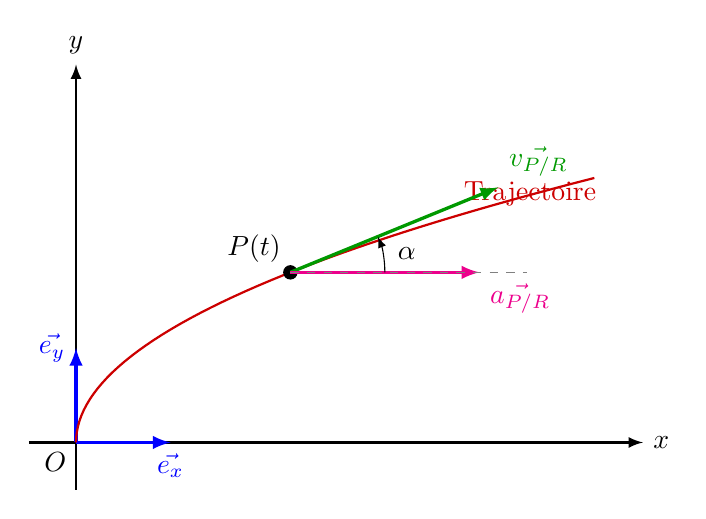
\begin{tikzpicture}[scale=1.2, >=latex]
    \draw[->, thick] (-0.5, 0) -- (6, 0) node[right] {$x$};
    \draw[->, thick] (0, -0.5) -- (0, 4) node[above] {$y$};
    \node[below left] at (0,0) {$O$};

    \draw[->, very thick, blue] (0,0) -- (1,0) node[below] {$\vec{e_x}$};
    \draw[->, very thick, blue] (0,0) -- (0,1) node[left] {$\vec{e_y}$};

    \draw[thick, red!80!black, domain=0:2.8, samples=50] plot ({0.7*\x*\x}, {\x});
    \node[red!80!black, above right] at (4, 2.4) {Trajectoire};

    \coordinate (P) at (2.268, 1.8);
    \filldraw[black] (P) circle (2pt) node[above left] {$P(t)$};

    \draw[->, very thick, green!60!black] (P) -- ++(2.2, 0.9) node[above right] {$\vec{v_{P/R}}$};
    \draw[->, very thick, magenta] (P) -- ++(2.0, 0) node[below right] {$\vec{a_{P/R}}$};

    \draw[dashed, gray] (P) -- ++(2.5, 0);
    \draw[->] (P) ++(1.0, 0) arc (0:22.2:1.0);
    \node at (3.5, 2.0) {$\alpha$};
\end{tikzpicture}
\end{center}

\subsection*{c) Norme de la vitesse, nature du mouvement, composantes de Frenet}

\subsubsection*{1- Norme de la vitesse et nature du mouvement}
\begin{sonucbox}
$$ ||\vec{v_{P/R}}|| = \sqrt{v_x^2 + v_y^2} = \sqrt{(2ct)^2 + b^2} = \sqrt{4c^2t^2 + b^2} $$
\end{sonucbox}
Pour la nature du mouvement, on étudie la dérivée du \emph{carré} de la norme (pas de racine à dériver) :
$$ \frac{d||\vec{v}||^2}{dt} = \frac{d}{dt}\left(4c^2t^2 + b^2\right) = 8c^2t $$
D'autre part, $\dfrac{d||\vec{v}||^2}{dt} = 2\,||\vec{v}||\,\dfrac{d||\vec{v}||}{dt}$, donc :
$$ \frac{d||\vec{v}||}{dt} = \frac{8c^2t}{2\,||\vec{v}||} = \frac{4c^2t}{\sqrt{4c^2t^2 + b^2}} $$
Cette quantité est du signe de $t$ (car $c>0$) : elle est strictement positive pour $t>0$.
\begin{sonucbox}
Le mouvement est \textbf{accéléré} pour $t>0$. À $t=0$ on a $\vec{a}\cdot\vec{v}=0$ : la norme de la vitesse est alors minimale ($||\vec{v}||=b$).
\end{sonucbox}

\subsubsection*{2- Composante tangentielle $a_t$}
Le vecteur unitaire tangent est $\vec{T} = \dfrac{\vec{v}}{||\vec{v}||}$, et $a_t$ est la projection de $\vec{a}$ sur $\vec{T}$. On calcule d'abord le produit scalaire :
$$ \vec{a}\cdot\vec{v} = (2c)(2ct) + 0\cdot b = 4c^2t $$
puis :
$$ a_t = \vec{a}\cdot\vec{T} = \frac{\vec{a}\cdot\vec{v}}{||\vec{v}||} $$
\begin{sonucbox}
$$ a_t = \frac{4c^2t}{\sqrt{4c^2t^2 + b^2}} $$
\end{sonucbox}
On retrouve bien $a_t = \dfrac{d||\vec{v}||}{dt}$, comme attendu.

\subsubsection*{3- Composante normale $a_n$ (par le produit vectoriel)}
Comme $||\vec{a}\times\vec{v}|| = ||\vec{a}||\,||\vec{v}||\sin\theta$ où $\theta$ est l'angle entre $\vec{a}$ et $\vec{T}$, on a $a_n = ||\vec{a}||\sin\theta = \dfrac{||\vec{a}\times\vec{v}||}{||\vec{v}||}$. On calcule :
$$ \vec{a}\times\vec{v} = \begin{pmatrix} 2c \\ 0 \\ 0 \end{pmatrix}\times\begin{pmatrix} 2ct \\ b \\ 0 \end{pmatrix} = \begin{pmatrix} 0\cdot 0 - 0\cdot b \\ 0\cdot 2ct - 2c\cdot 0 \\ 2c\cdot b - 0\cdot 2ct \end{pmatrix} = \begin{pmatrix} 0 \\ 0 \\ 2bc \end{pmatrix} $$
d'où $||\vec{a}\times\vec{v}|| = 2bc$ et :
\begin{sonucbox}
$$ a_n = \frac{||\vec{a}\times\vec{v}||}{||\vec{v}||} = \frac{2bc}{\sqrt{4c^2t^2 + b^2}} $$
\end{sonucbox}
\textbf{Vérification} avec $a_t^2 + a_n^2 = ||\vec{a}||^2$ :
\begin{align*}
a_t^2 + a_n^2 &= \frac{16c^4t^2}{4c^2t^2 + b^2} + \frac{4b^2c^2}{4c^2t^2 + b^2} \\
&= \frac{4c^2\left(4c^2t^2 + b^2\right)}{4c^2t^2 + b^2} = 4c^2 = ||\vec{a}||^2 \quad \checkmark
\end{align*}

\subsection*{d) Angle $\alpha$ et méthode géométrique}

\subsubsection*{1- Calcul de $\cos\alpha$}
Avec $\alpha = (\vec{e_x}, \vec{v_{P/R}})$, le produit scalaire donne $\vec{e_x}\cdot\vec{v} = ||\vec{e_x}||\,||\vec{v}||\cos\alpha = ||\vec{v}||\cos\alpha$. D'autre part $\vec{e_x}\cdot\vec{v} = v_x = 2ct$. Donc :
\begin{sonucbox}
$$ \cos\alpha = \frac{2ct}{\sqrt{4c^2t^2 + b^2}} $$
\end{sonucbox}
De même, $\vec{e_y}\cdot\vec{v} = v_y = b$ et $\vec{e_y}$ fait l'angle $\frac{\pi}{2}-\alpha$ avec $\vec{v}$, donc $\sin\alpha = \dfrac{v_y}{||\vec{v}||} = \dfrac{b}{\sqrt{4c^2t^2 + b^2}}$. On vérifie : $\cos^2\alpha + \sin^2\alpha = \dfrac{4c^2t^2 + b^2}{4c^2t^2 + b^2} = 1$.

\subsubsection*{2- Retrouver $a_n$ avec $||\vec{a}||$ et $\alpha$}
Le vecteur $\vec{T}$ est dirigé selon $\vec{v}$, donc $\vec{T} = \cos\alpha\,\vec{e_x} + \sin\alpha\,\vec{e_y}$. Le vecteur $\vec{N}$ est perpendiculaire à $\vec{T}$ et orienté vers l'intérieur de la concavité (donc avec une composante positive sur $\vec{e_x}$) :
$$ \vec{N} = \sin\alpha\,\vec{e_x} - \cos\alpha\,\vec{e_y} $$
On en déduit $\vec{e_x} = \cos\alpha\,\vec{T} + \sin\alpha\,\vec{N}$, ce que l'on vérifie directement :
$$ \cos\alpha\,(\cos\alpha,\sin\alpha) + \sin\alpha\,(\sin\alpha,-\cos\alpha) = (\cos^2\alpha+\sin^2\alpha,\; 0) = (1,\,0) \quad\checkmark $$
Comme $\vec{a} = ||\vec{a}||\,\vec{e_x} = 2c\,\vec{e_x}$ :
$$ \vec{a} = 2c\cos\alpha\,\vec{T} + 2c\sin\alpha\,\vec{N} \quad\Longrightarrow\quad a_t = ||\vec{a}||\cos\alpha,\quad a_n = ||\vec{a}||\sin\alpha $$
\begin{sonucbox}
$$ a_n = 2c\cdot\frac{b}{\sqrt{4c^2t^2 + b^2}} = \frac{2bc}{\sqrt{4c^2t^2 + b^2}} $$
\end{sonucbox}
On retrouve exactement le résultat de la question c-3. De plus, $a_t = 2c\cdot\dfrac{2ct}{\sqrt{4c^2t^2+b^2}} = \dfrac{4c^2t}{\sqrt{4c^2t^2+b^2}}$ coïncide avec c-2.

\begin{sonucbox}
\textbf{Récapitulatif de l'exercice 1}
\begin{center}
\renewcommand{\arraystretch}{1.8}
\begin{tabular}{|c|c|}
\hline
$\vec{v_{P/R}}$ & $2ct\,\vec{e_x} + b\,\vec{e_y}$ \\
\hline
$\vec{a_{P/R}}$ & $2c\,\vec{e_x}$ \\
\hline
$||\vec{v}||$ & $\sqrt{4c^2t^2+b^2}$ \\
\hline
$a_t$ & $\dfrac{4c^2t}{\sqrt{4c^2t^2+b^2}}$ \\
\hline
$a_n$ & $\dfrac{2bc}{\sqrt{4c^2t^2+b^2}}$ \\
\hline
\end{tabular}
\end{center}
\end{sonucbox}

\newpage

\section*{Exercice 2 : Mouvement plan circulaire uniforme}

\begin{theoriebox}{Alternatif Yöntemler}
\begin{itemize}
    \item \textbf{Tek kosinüs formu :} $A\cos\varphi + B\sin\varphi = R_0\cos(\varphi-\delta)$ yazılabilir; burada $R_0=\sqrt{A^2+B^2}$, $\cos\delta = A/R_0$, $\sin\delta = B/R_0$. Bu şekilde türevler ve normlar çok kısalır.
    \item \textbf{Kutupsal bileşenler :}
    $$ v_\rho = \dot\rho,\quad v_\varphi = \rho\dot\varphi,\quad a_\rho = \ddot\rho - \rho\dot\varphi^2,\quad a_\varphi = 2\dot\rho\dot\varphi + \rho\ddot\varphi $$
    \item \textbf{Çarpım-toplam dönüşümü :} $\cos u\cos v=\frac12\left[\cos(u+v)+\cos(u-v)\right]$ ve $\sin v\cos u = \frac12\left[\sin(v+u)+\sin(v-u)\right]$ özdeşlikleri ile $x(t)$ ve $y(t)$ doğrudan çember parametrizasyonuna döner.
    \item \textbf{Düzgün dairesel hareket :} $v=R\Omega$ ve $a=R\Omega^2=\frac{v^2}{R}$ ($\Omega$: çember üzerindeki açısal hız).
\end{itemize}
\end{theoriebox}

Dans le repère $R(O,\vec{e_x},\vec{e_y})$, le point $P$ a pour coordonnées polaires :
$$ \rho(t) = A\cos\varphi + B\sin\varphi, \qquad \varphi(t) = \omega t \qquad (A,B,\omega>0) $$

\textbf{Mise en forme préliminaire.} Posons $R_0 = \sqrt{A^2+B^2}$ et l'angle $\delta\in\left]0,\frac{\pi}{2}\right[$ tel que $\cos\delta = \frac{A}{R_0}$ et $\sin\delta = \frac{B}{R_0}$ (c'est possible car $\left(\frac{A}{R_0}\right)^2 + \left(\frac{B}{R_0}\right)^2 = 1$ et $A,B>0$). Alors :
$$ \rho = R_0\left(\cos\delta\cos\varphi + \sin\delta\sin\varphi\right) = R_0\cos(\varphi - \delta) = R_0\cos(\omega t - \delta) $$

\subsection*{a) Vitesse en coordonnées cylindriques et nature du mouvement}
Le vecteur position est $\vec{OP} = \rho\,\vec{e_\rho}$, donc $\vec{v_{P/R}} = \dot\rho\,\vec{e_\rho} + \rho\,\dot\varphi\,\vec{e_\varphi}$. Avec $\dot\varphi = \omega$ constant, on dérive $\rho(t) = R_0\cos(\omega t-\delta)$ :
\begin{align*}
v_\rho &= \frac{d\rho}{dt} = -R_0\,\omega\sin(\omega t - \delta) \\
v_\varphi &= \rho\,\dot\varphi = R_0\,\omega\cos(\omega t - \delta)
\end{align*}
\begin{sonucbox}
$$ \vec{v_{P/R}} = -R_0\omega\sin(\omega t-\delta)\,\vec{e_\rho} + R_0\omega\cos(\omega t-\delta)\,\vec{e_\varphi} $$
\end{sonucbox}
Pour revenir à $A$ et $B$, on développe :
\begin{align*}
\cos(\omega t-\delta) &= \cos\omega t\cos\delta + \sin\omega t\sin\delta = \frac{A\cos\omega t + B\sin\omega t}{R_0} \\
\sin(\omega t-\delta) &= \sin\omega t\cos\delta - \cos\omega t\sin\delta = \frac{A\sin\omega t - B\cos\omega t}{R_0}
\end{align*}
d'où la forme équivalente :
$$ v_\rho = \omega\left(B\cos\omega t - A\sin\omega t\right), \qquad v_\varphi = \omega\left(A\cos\omega t + B\sin\omega t\right) $$
Calcul de la norme :
\begin{align*}
||\vec{v}||^2 &= v_\rho^2 + v_\varphi^2 \\
&= R_0^2\omega^2\left[\sin^2(\omega t-\delta) + \cos^2(\omega t-\delta)\right] \\
&= R_0^2\omega^2
\end{align*}
\begin{sonucbox}
$$ ||\vec{v_{P/R}}|| = \omega\sqrt{A^2+B^2} = \text{cste} \quad\Longrightarrow\quad \text{mouvement \textbf{uniforme}.} $$
\end{sonucbox}
La vitesse est constante en norme mais pas en direction : le point tourne. Le mouvement sera donc \textbf{circulaire uniforme} si la trajectoire est un cercle, ce que l'on montre en c).

\subsection*{b) Accélération en coordonnées cylindriques}
On a $\dot\varphi=\omega$ et $\ddot\varphi = 0$. On dérive $v_\rho$ pour obtenir $\ddot\rho$ :
$$ \ddot\rho = \frac{d}{dt}\left[-R_0\omega\sin(\omega t-\delta)\right] = -R_0\omega^2\cos(\omega t-\delta) = -\omega^2\rho $$
On applique les formules de l'accélération en coordonnées polaires :
\begin{align*}
a_\rho &= \ddot\rho - \rho\dot\varphi^2 = -\omega^2\rho - \omega^2\rho = -2\omega^2\rho = -2\omega^2R_0\cos(\omega t-\delta) \\
a_\varphi &= 2\dot\rho\,\dot\varphi + \rho\,\ddot\varphi = 2\omega\left(-R_0\omega\sin(\omega t-\delta)\right) + 0 = -2\omega^2R_0\sin(\omega t-\delta)
\end{align*}
\begin{sonucbox}
$$ \vec{a_{P/R}} = -2\omega^2R_0\cos(\omega t-\delta)\,\vec{e_\rho} - 2\omega^2R_0\sin(\omega t-\delta)\,\vec{e_\varphi} $$
\end{sonucbox}
En revenant à $A$ et $B$ avec les relations de la question a) :
$$ a_\rho = -2\omega^2\left(A\cos\omega t+B\sin\omega t\right), \qquad a_\varphi = 2\omega^2\left(B\cos\omega t - A\sin\omega t\right) $$
Norme :
\begin{align*}
||\vec{a}||^2 &= a_\rho^2 + a_\varphi^2 \\
&= 4\omega^4R_0^2\left[\cos^2(\omega t-\delta)+\sin^2(\omega t-\delta)\right] = 4\omega^4R_0^2
\end{align*}
\begin{sonucbox}
$$ ||\vec{a_{P/R}}|| = 2\omega^2\sqrt{A^2+B^2} = \text{cste} $$
\end{sonucbox}

\subsection*{c) Équation cartésienne de la trajectoire}
On calcule $x=\rho\cos\varphi$ et $y=\rho\sin\varphi$ avec $\rho=R_0\cos(\varphi-\delta)$, en utilisant les formules de linéarisation :
$$ \cos u\cos v = \tfrac{1}{2}\left[\cos(u+v)+\cos(u-v)\right], \qquad \sin v\cos u = \tfrac{1}{2}\left[\sin(v+u)+\sin(v-u)\right] $$
avec $u=\varphi-\delta$ et $v=\varphi$ :
\begin{align*}
x &= R_0\cos(\varphi-\delta)\cos\varphi = \frac{R_0}{2}\left[\cos(2\varphi-\delta) + \cos\delta\right] = \frac{A}{2} + \frac{R_0}{2}\cos(2\omega t-\delta) \\
y &= R_0\cos(\varphi-\delta)\sin\varphi = \frac{R_0}{2}\left[\sin(2\varphi-\delta) + \sin\delta\right] = \frac{B}{2} + \frac{R_0}{2}\sin(2\omega t-\delta)
\end{align*}
(on a utilisé $R_0\cos\delta=A$ et $R_0\sin\delta=B$). Donc :
$$ x - \frac{A}{2} = \frac{R_0}{2}\cos(2\omega t - \delta), \qquad y - \frac{B}{2} = \frac{R_0}{2}\sin(2\omega t - \delta) $$
En élevant au carré et en sommant :
\begin{align*}
\left(x-\frac{A}{2}\right)^2 + \left(y-\frac{B}{2}\right)^2 &= \frac{R_0^2}{4}\left[\cos^2(2\omega t-\delta) + \sin^2(2\omega t-\delta)\right] = \frac{R_0^2}{4}
\end{align*}
\begin{sonucbox}
$$ \left(x-\frac{A}{2}\right)^2 + \left(y-\frac{B}{2}\right)^2 = \frac{A^2+B^2}{4} $$
\end{sonucbox}
C'est un \textbf{cercle} de centre $C\left(\frac{A}{2},\frac{B}{2}\right)$ et de rayon $\dfrac{\sqrt{A^2+B^2}}{2}$. Il passe par l'origine $O$, car $\left(0-\frac{A}{2}\right)^2 + \left(0-\frac{B}{2}\right)^2 = \frac{A^2+B^2}{4}$. De plus, l'angle $2\omega t-\delta$ montre que $P$ parcourt ce cercle à la vitesse angulaire $2\omega$ autour de $C$.

\textbf{Vérification par une deuxième méthode.} On multiplie $\rho = A\cos\varphi + B\sin\varphi$ par $\rho$ :
$$ \rho^2 = A\,\rho\cos\varphi + B\,\rho\sin\varphi \quad\Longrightarrow\quad x^2 + y^2 = Ax + By $$
Puis on complète les carrés :
$$ \left(x^2 - Ax + \frac{A^2}{4}\right) + \left(y^2 - By + \frac{B^2}{4}\right) = \frac{A^2}{4} + \frac{B^2}{4} \;\Longrightarrow\; \left(x-\frac{A}{2}\right)^2 + \left(y-\frac{B}{2}\right)^2 = \frac{A^2+B^2}{4} $$
On retrouve la même équation.

\begin{center}
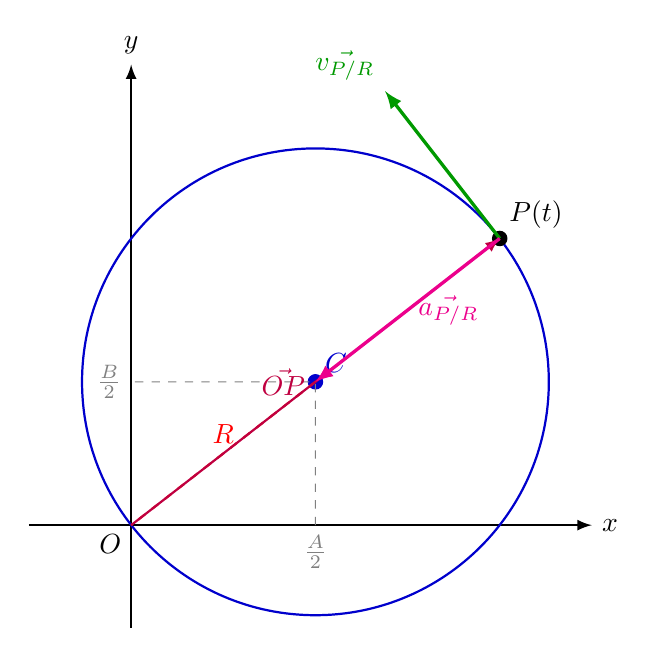
\begin{tikzpicture}[scale=1.3, >=latex]
    \draw[->, thick] (-1, 0) -- (4.5, 0) node[right] {$x$};
    \draw[->, thick] (0, -1) -- (0, 4.5) node[above] {$y$};
    \node[below left] at (0,0) {$O$};

    \coordinate (C) at (1.8, 1.4);
    \draw[thick, blue!80!black] (C) circle (2.28);
    \filldraw[blue!80!black] (C) circle (2pt) node[above right] {$C$};
    \draw[dashed, gray] (1.8, 0) node[below] {$\frac{A}{2}$} -- (C) -- (0, 1.4) node[left] {$\frac{B}{2}$};
    \draw[thick, dashed, red] (C) -- (0,0) node[midway, above] {$R$};

    \coordinate (P) at (3.6, 2.8);
    \filldraw[black] (P) circle (2pt) node[above right] {$P(t)$};
    \draw[->, thick, purple] (0,0) -- (P) node[midway, left] {$\vec{OP}$};
    \draw[->, very thick, green!60!black] (P) -- ++(-1.12, 1.44) node[above left] {$\vec{v_{P/R}}$};
    \draw[->, very thick, magenta] (P) -- (C) node[midway, right] {$\vec{a_{P/R}}$};
\end{tikzpicture}
\end{center}

\subsection*{d) Rayon à partir de $||\vec{a_{P/R}}||$}
D'après a), le mouvement est uniforme : $||\vec{v}||$ est constante, donc $a_t = \dfrac{d||\vec{v}||}{dt} = 0$. L'accélération est alors purement normale :
$$ ||\vec{a}|| = a_n = \frac{v^2}{R} \quad\Longrightarrow\quad R = \frac{v^2}{||\vec{a}||} $$
On remplace $v = \omega R_0$ et $||\vec{a}|| = 2\omega^2R_0$ :
\begin{sonucbox}
$$ R = \frac{\omega^2R_0^2}{2\omega^2R_0} = \frac{R_0}{2} = \frac{\sqrt{A^2+B^2}}{2} $$
\end{sonucbox}
\textbf{Cohérence avec c) :} le point décrit le cercle de rayon $R$ à la vitesse angulaire $2\omega$, donc
$$ v = R\cdot 2\omega = \frac{R_0}{2}\cdot 2\omega = \omega R_0 \qquad\text{et}\qquad a = R\,(2\omega)^2 = \frac{R_0}{2}\cdot 4\omega^2 = 2\omega^2R_0 $$
ce qui coïncide avec les résultats de a) et b). Le rayon obtenu ici est bien celui de la question c).

\begin{sonucbox}
\textbf{Récapitulatif de l'exercice 2}
\begin{center}
\renewcommand{\arraystretch}{1.8}
\begin{tabular}{|c|c|}
\hline
$||\vec{v}||$ & $\omega\sqrt{A^2+B^2}$ (mouvement uniforme) \\
\hline
$||\vec{a}||$ & $2\omega^2\sqrt{A^2+B^2}$ \\
\hline
Trajectoire & cercle de centre $C\left(\frac{A}{2},\frac{B}{2}\right)$ passant par $O$ \\
\hline
Rayon & $R=\dfrac{\sqrt{A^2+B^2}}{2}$ \\
\hline
Vitesse angulaire sur le cercle & $2\omega$ \\
\hline
\end{tabular}
\end{center}
\end{sonucbox}

\end{document}
